\documentclass[a4paper, 11pt]{scrartcl}
\usepackage[utf8]{inputenc}
\usepackage{xcolor}
\usepackage{graphicx}
\graphicspath{{./figures/}}

\title{Assignment 1}
\author{Alina Mokrova\\
				01325014
				\and
				Levente	Slajchó\\
				01634250
				\and
				Maximilian Walterskirchen\\
				11809927
				\and
				Leminh Nguyen\\
				11945068}
\date{\today}

\begin{document}

\maketitle

\section{Analysis and criticism}

\subsection{Analysis of the infographic}

% corrected
The infographic \textit{Nutritional Values} by Dan Mariglio in
Figure~\ref{assignmentGraphic} pictures the nutritional comparison between
processed and natural/wholesome food. The author visualizes three different
infographics for the different food categories; the first graph compares the
cost per calorie, another one contrasts the calories per \textit{100g} and the
last graphic shows how much sugar is contained in \textit{100g}. The author
gives the example that wholesome food is more expensive since the ratio of value
to calorie for an apple is higher compared to a bag of potato chips. Mariglio
based his visualizations on the layout of common supermarkets and suggests the
reader sticking to the periphery of the supermarket to find the natural food.
Processed food containing the most calories by weight is located at the centre
of the grocery store.

\subsection{Criticism of the visual design}

% corrected
In this section, the three infographics in Figuren~\ref{assignmentGraphic} will
be criticised according to the visual design principles from the lecture notes.
These design principles were defined by Edward Tufte\cite{Tufte2001}. Since the
three illustrations are very similar in design, the criticism will cover its
general design principle choices.

\subsubsection{Perception and cognition}


% corrected
On first sight of the infographics as a viewer, there is no immediate
understanding of the given information. There are too many bright colours which
can distract the viewer to localize the main message or information of the
visual design. Further, the visual design carries no preattentive attributes,
except the black food labels but many of them are obscured by other visual
components or are drowning in the variety of colours which are more distracting
than communication the information with clarity.  Thus, on first sight, the
infographics are flawed for immediate perception.

% corrected
The reasons which cause the infographics to be unsatisfactory are the poorly
chosen design principles by the author. Instead of the \textit{preattentive
processing paradigm}, the author uses the data-driven, Bottom-up approach.
Therefore, the graphs should be perceived with the visual processing paradigm
and require from the viewer an attentive perception and parallel processing to
extract low-level properties of the visual scene. The attentive approach is slow
to perceive and viewers easily forget the main message and essential information
of the infographic. Furthermore, the visual representation is not friendly for
viewers who might suffer from colour blindness since the author uses a wide
subset of colours in his visual design.

\subsubsection{Deficiency of design priniciples by Edward Tufte}

\textbf{Principles of Graphical Excellence.} 

% Complex ideas communicated with clarity, precision and efficiency.
% The viewer grasps the ideas of the visualization quick with the least amount of ink in the smallest space

\textbf{Principles of Graphical Integrity.}

% Lie Factor
% Clear detailed and labelled
% show data variation, not design variation
% not exceed the number of dimensions of the data
% Principles of Graphical Integrity (Tufte principles of design)
% The food graphical components obscure the actual information and data -> hard to perceive actual infographic
% The graphic in 3 dimensions which makes itway more complex than it is

\textbf{Principles of Data Graphics.}

% Show me the numbers:
% ‘Above all show the data’
% Ink should present new information
% Elimination of non-data ink without loss of the data
% The elegance of visual design, defined by reached state where no elements cannot be removed and not the other way around of nothing to add
% Deemphasize non-data ink
% Push non-data ink into the background (supermarket blueprint)
% Display data in the foreground
% Nothing stands out since data-ink and non-data ink are given the same weight
% The viewers' eyes are drawn to contrast found in the 3d components which leads the reader from the actual data
% Different colours even though the same dataset leads the reader to think the difference it dataset
% Chartjunk 

% `A good graph is quiet and lets the data tell their story clearly and
% completely.`-Wainer, 1997
% Tufte Design Principles 
% 1. Above all else show the data 
% 2. Maximize the data-ink ratio 
% 3. Erase non-data-ink 
% 4. Erase redundant data-ink 
% 5. Maximize data density, within reason (Data density = number of entries/area of data graphic) 
% 6. Revise and edit



% Rules by Stephen Few about using colour in charts and graphs

% Use different colours only when they correspond to differences of meaning
% in the data 
% here for example for the vegetables multiple colours are used
% although that's not necessary

% To guarantee that most people who are colourblind can distinguish groups of data
% that are colour-coded, avoid using a combination of red and green in the same
% display.

% Use soft natural colours to display most information and bright and/or dark
% colours to highlight information that requires greater attention

\section{Assessment of redesign}
\section{Assessment of redesign}

How we decided to redesign the infographic:

\begin{itemize}
	\item \textbf{Deemphasize the non data-ink:} The original graphic has a very low data-ink ratio. Visual representation of the groceries in the graphics is totally unnecessary, since they are labeled with text too. About 60\% of the graphics are non-data ink, which causes a very low data-ink ratio 
    \item \textbf{Deemphasize the layout of the grocery story} supermarket blueprint/floor-plan in bright grey scales to deemphasize
		it's value and possibily to overshadow the essential graphs
	\item augment the data-ink
    \item Preattentive processing
	\item declutter
	\item regroup the data
\end{itemize}

% Push non-data ink into the background (supermarket blueprint)
% Display data in the foreground

% link to appendix of new design


% link to appendix of new design

\bibliographystyle{ieeetr}
\bibliography{ivassignment}

\newpage
\clearpage
\section{Appendix}

\begin{figure}[h]
  \centering
	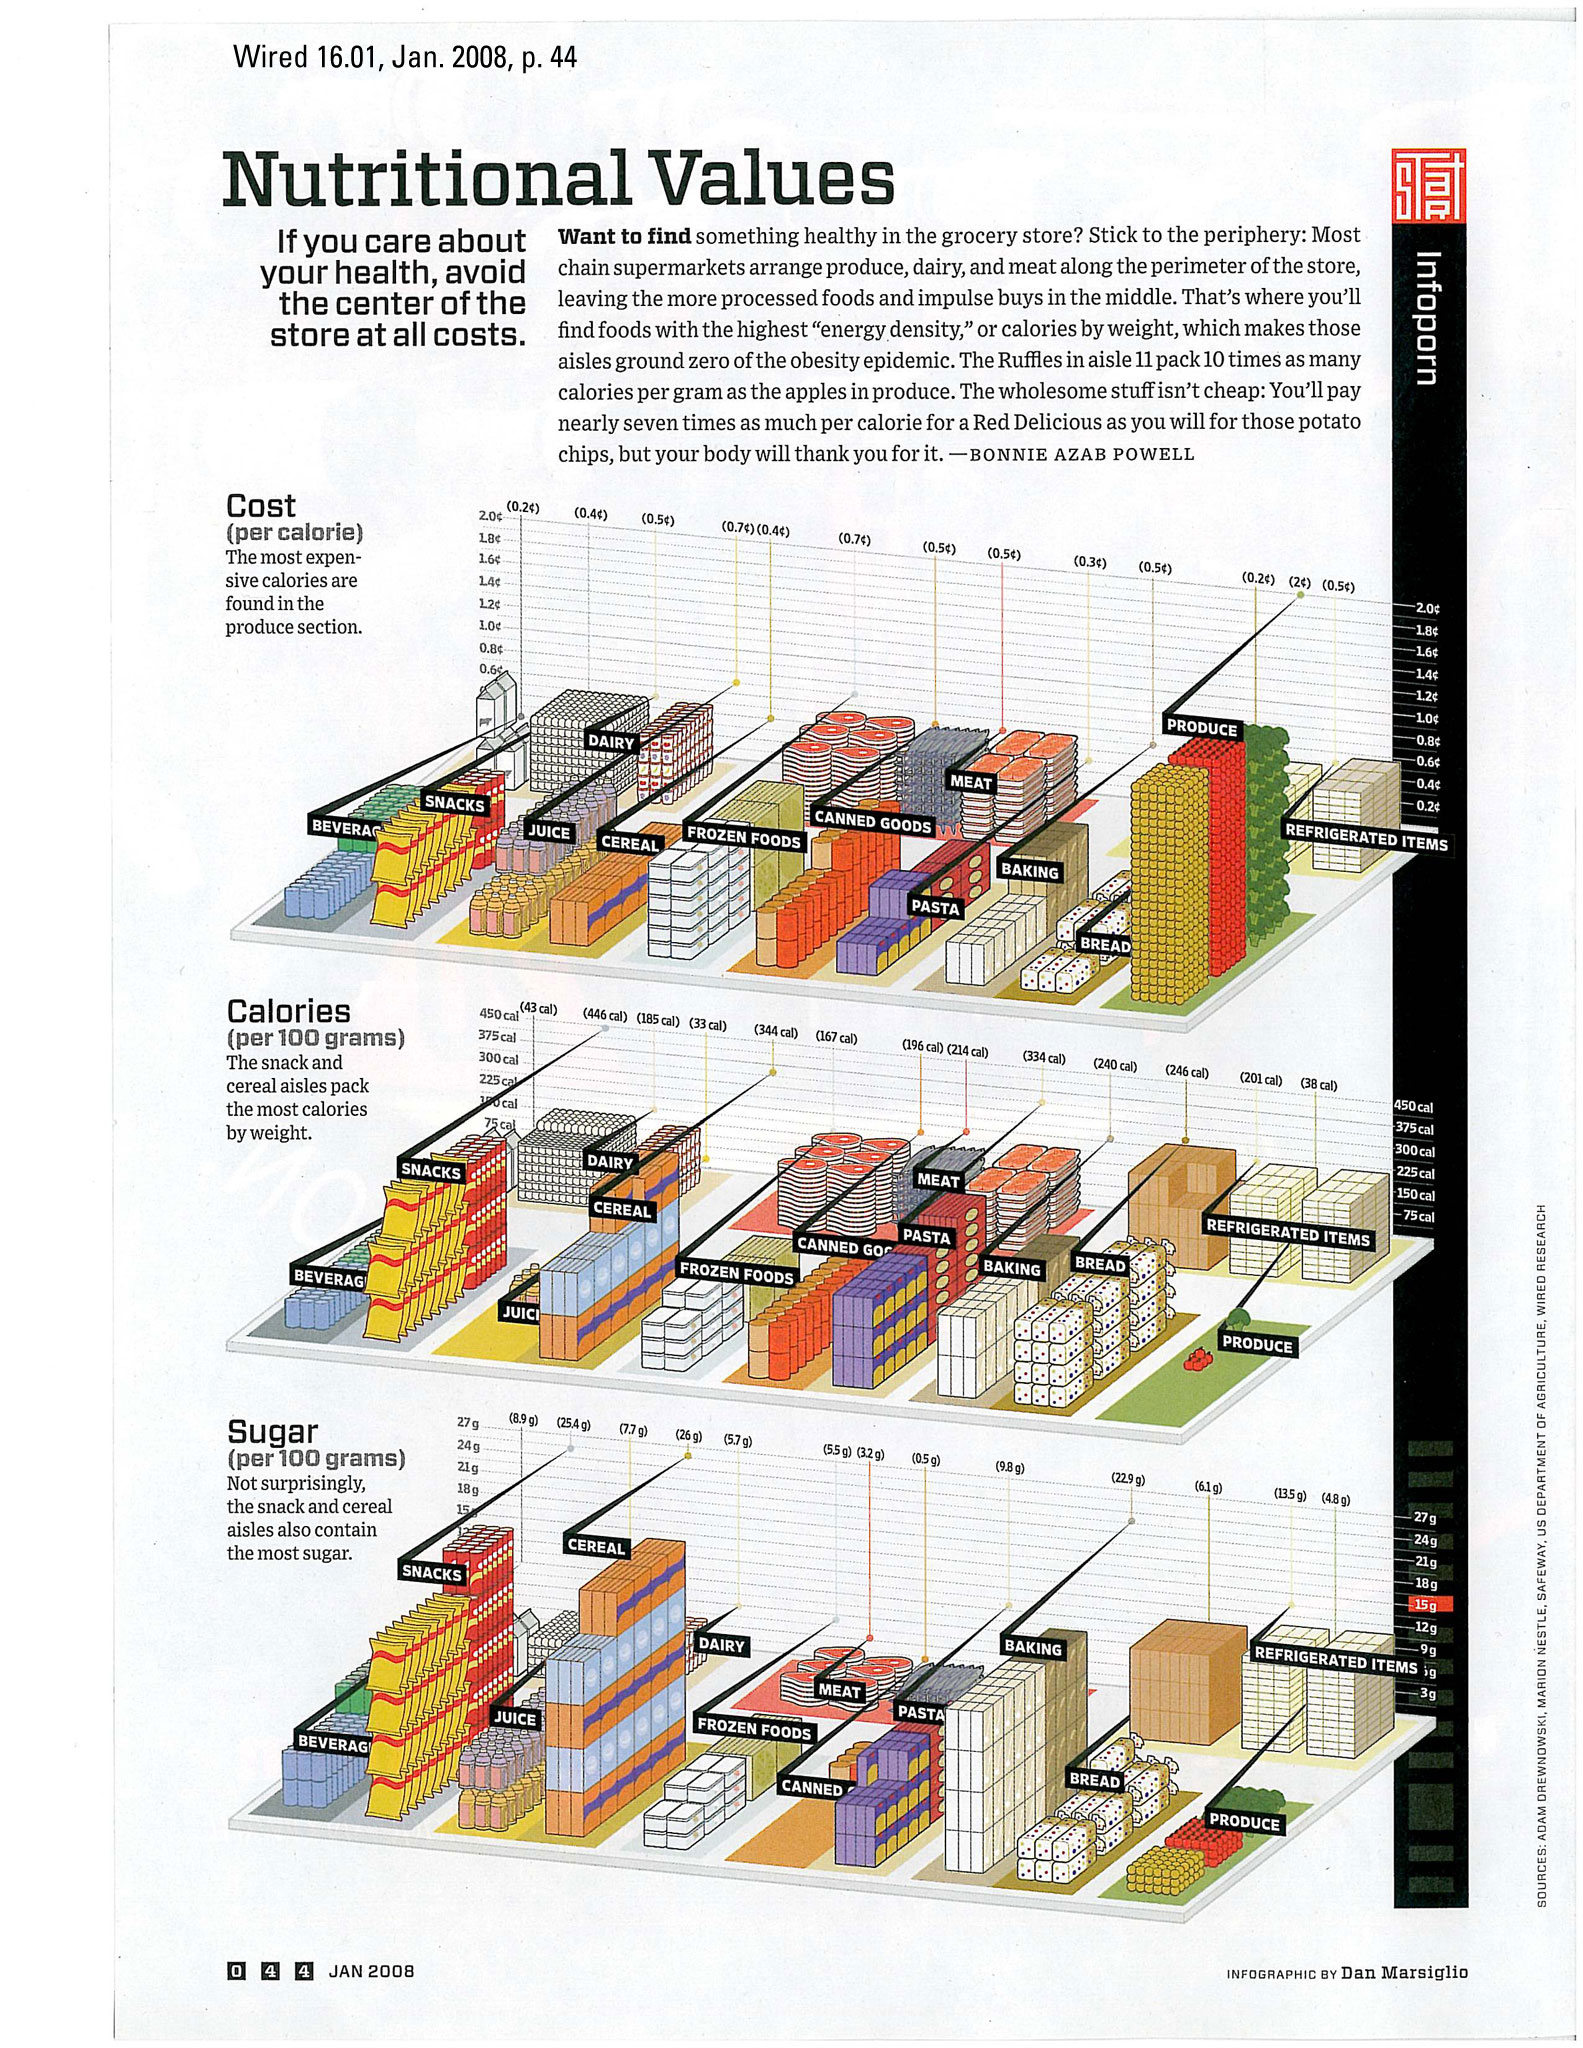
\includegraphics[scale=0.20]{assignmentGraphic.jpg}
  \caption{Dan Mariglio's infographic about nutritional values in a supermarket
	was assigned to our group to criticize.}
	\label{assignmentGraphic}
\end{figure}

\begin{figure}[h]
  \centering
	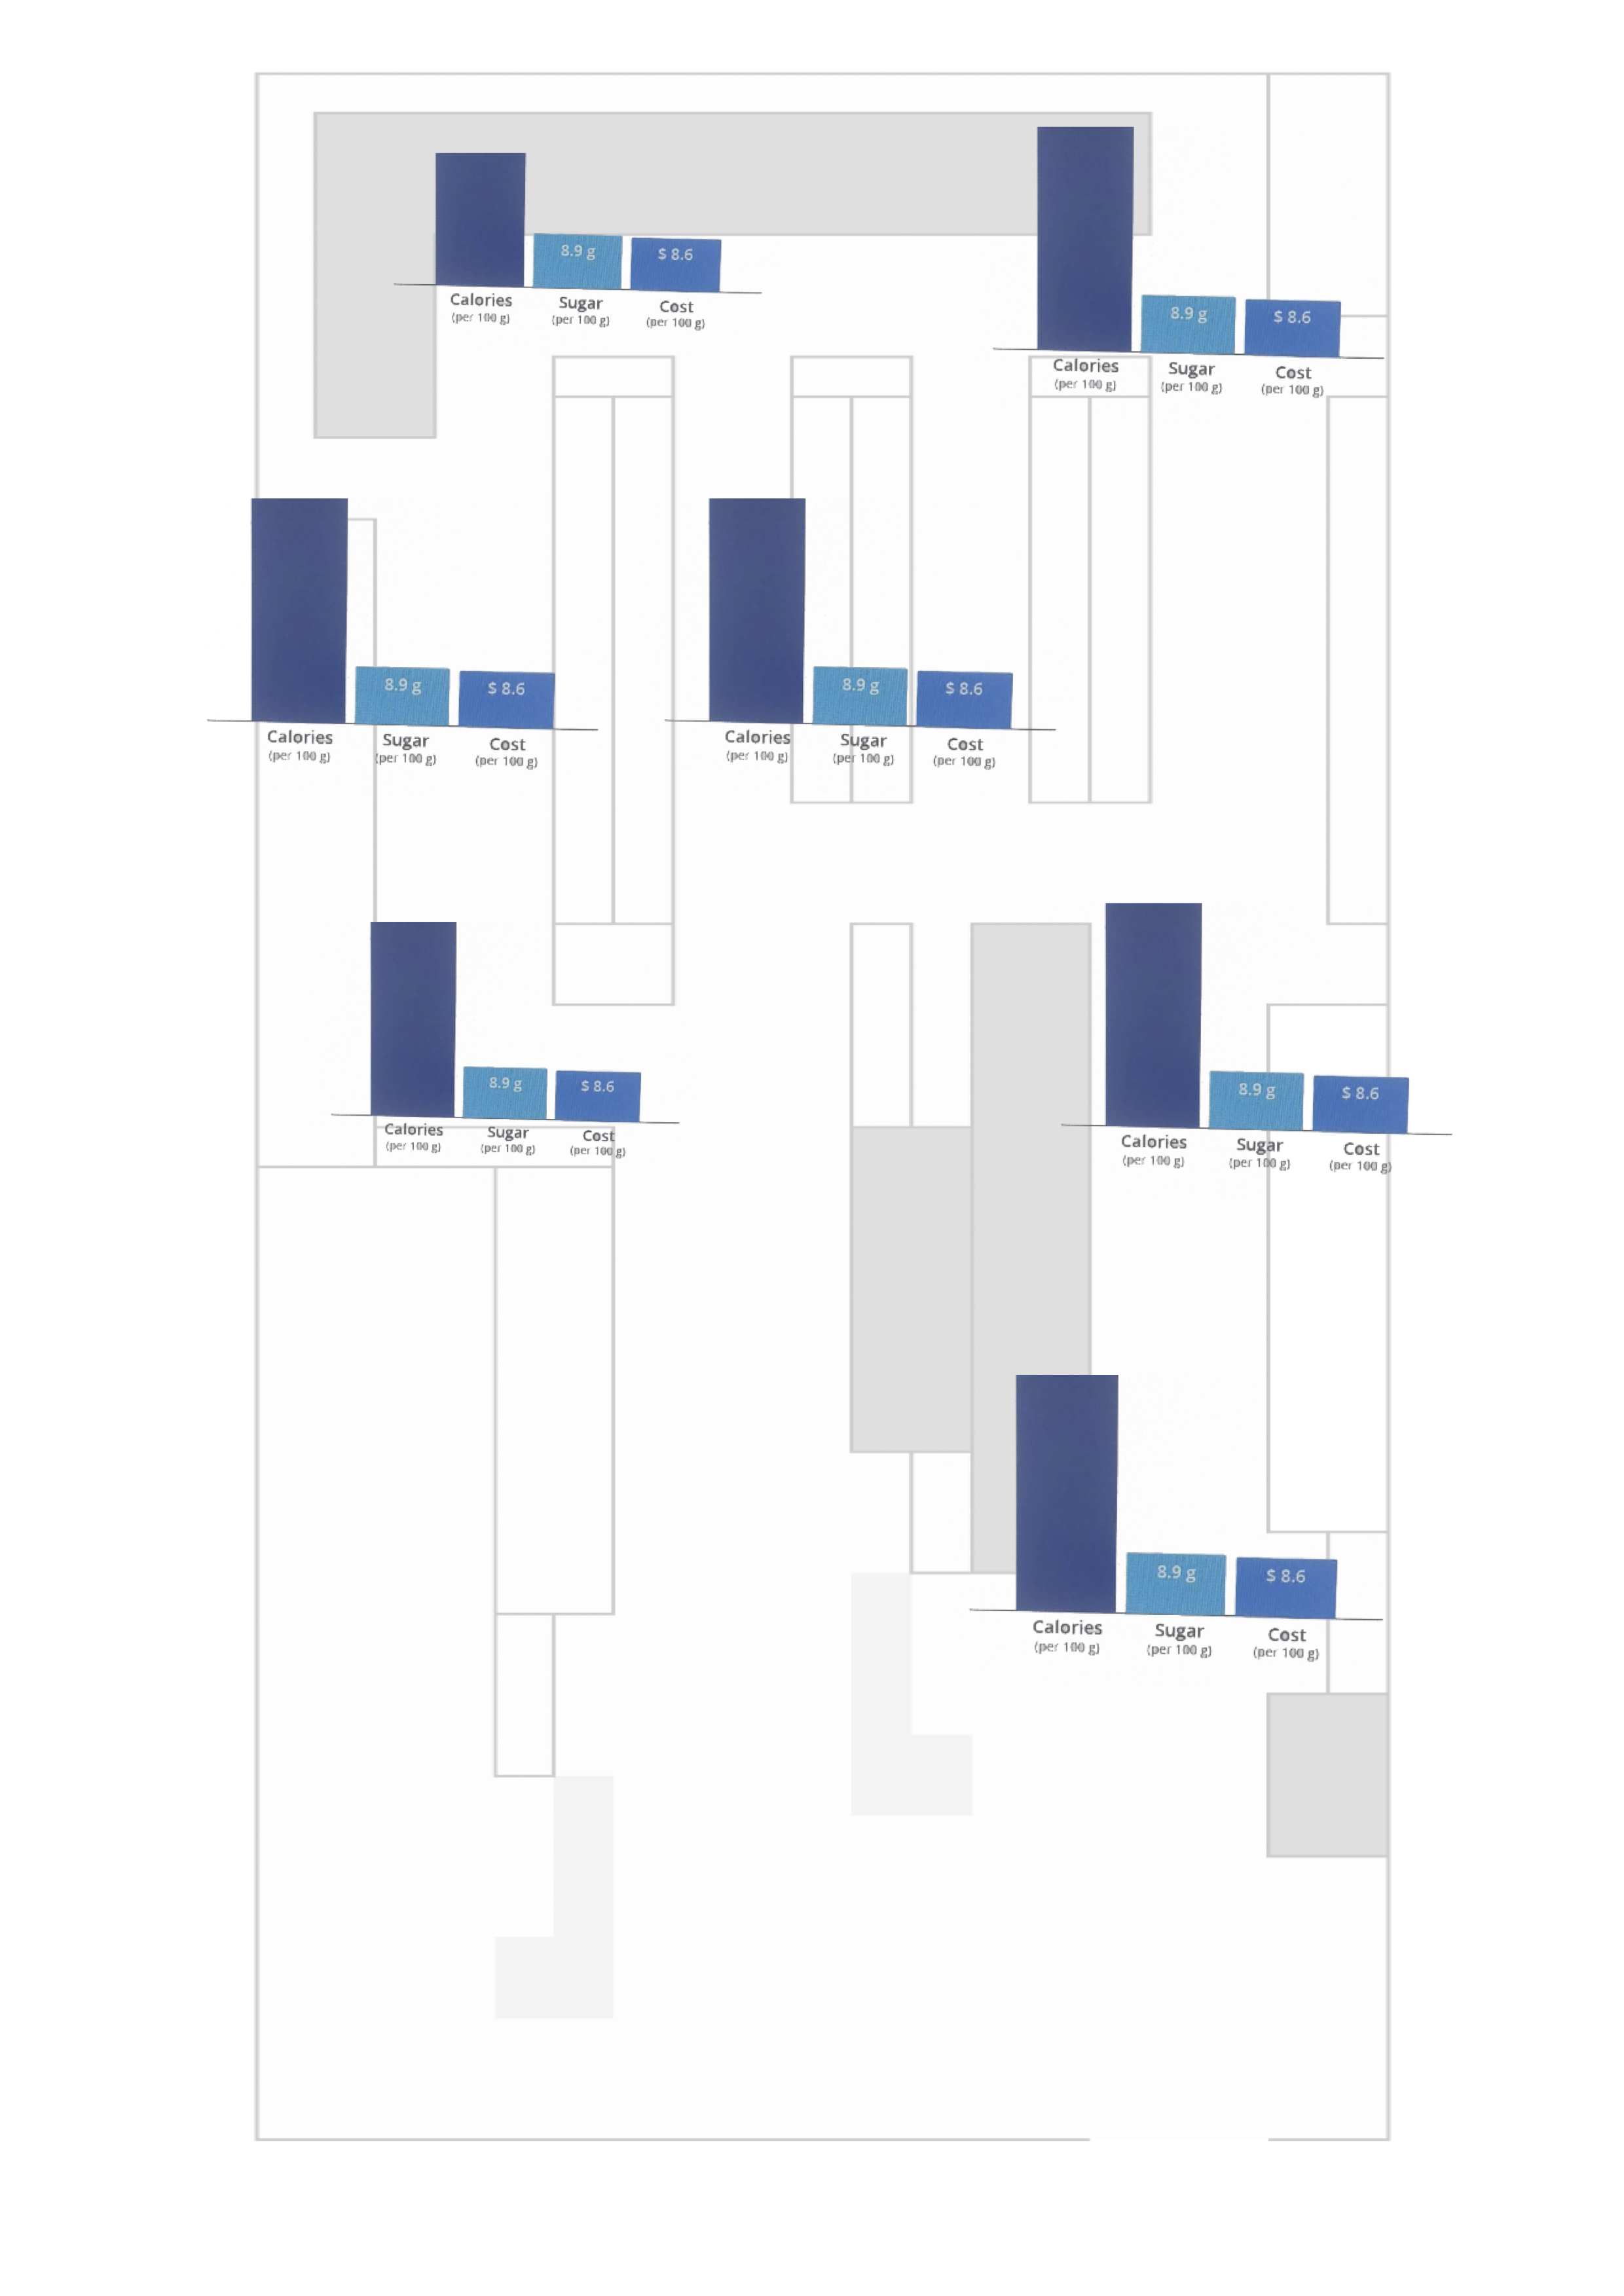
\includegraphics[scale=0.15]{redesignGraphic.jpg}
  \caption{Redesign Dan Mariglio's infographic about nutritional values in a
	supermarket. A \textit{.jpg} file will be provided in the submission folder.}
	\label{redesignGraphic}
\end{figure}

\end{document}
